

\section{A new Emulation Technique for Sensitivity Analysis
for SRAM FPGAs}
\label{intro}
% no \IEEEPARstart


The purpose of this work is  to  use the sensitivity specific bits to produce the highly accurate fault behavior as expected in the real-time testing environment. Because the work done in~\citep{souari2016towards} showed that if we consider the bits relative sensitivity --- the bits at "1" are more sensitive than the bits at "0", we get more realistic results, closer to the radiation based experiments. 

In this work, the signature is calculated that presents the faulty behavior of the computation. The new fault emulation technique is used --- the method is based on the bits relative sensitivity, and it's feature.  We observed that the signature computed by our sensitivity-based method are $98.47$\% closer for adder circuit and $99.49$ \% closer for the multiplier circuit to the radiation based signature.

This work is the extension of the previous work and make the following contributions. 


\textbf{Contributions:} \\

\begin{itemize}



\item{Developed a realistic fault emulation technique in the configuration memory
of FPGAs based system}.

\item{In this work, we propose a fault injection method by using relative sensitivity values between the bits features: e.g., bits belong to LUT at "0", bits belong to LUT at "1", bits belong to Non-LUT at "0", bits belong to Non-LUT at "1"}.

\item{Zero-signature has been derived by flipping the bits-at-1, bits-at-0, randomly, flipped the bits based on the relative sensitivity between bits-at-1, bits-at-0, and relative sensitivity between bits-status and their features}.
\end{itemize}


In order, to find the faulty behavior of the circuits for their early validation, we extracted the information from the arithmetic signatures in terms of zero-signatures. To emulate faults in the FPGA based design, we  developed a suitable fault injection method. The fault injection method is based on the relative sensitivity of the bits and bits features as well, i.e., the bits belong to look-up-table or non look-up-table bits. We observed that by considering the bits feature; we produced more realistic results closer to the real-time experiments. In this paper, we also provide the results if the sensitivity of the bits is not taking into consideration lead towards the deviated results for the real-time radiation experiment.




\section{Methodology}
\label{Methodology}

The emulation of SEUs in an FPGA is done by flipping the bit in the configuration memory by using the IP provided by the Xilinx named - SEM core~\citep{xilinx}. The emulation platform used in this work was designed for the radiation experiment~\citep{hobeika2014multi}. In this work, this platform is employed for the fault emulation. The platform comprises of two Artix-7 FPGAs. The "Reference-Board" comprises of the original design, e.g., 16-bit adder and 8-bit multiplier. The design under "Test-Board" is subjected to fault emulation.  

%The work adopted the emulation work also proposed in the~\cite{hobeika2013flight}.  The work described a completed automated methodology to emulate SEUs on an FPGA efficiently. The work presented in~\cite{hobeika2014multi} used the Artix-7 board for the emulation puposes. 


This work comprises of four-step:
\begin{itemize}
\item{Fault emulation platform: configuration and validation}
\item{Fault emulation: flip-at-1, flip-at-0, random fault injection, sensitivity aware, and sensitivity aware based on the bits feature}.
 %\item {High-level fault modelling}
\item{Result analysis and bit flip validation}.
\end{itemize}


\subsection{Identification of the Sensitivity bits}
\label{SE-bits}

I start working on this project from the identification of the bits (the bit address and the bit location). The identification of the bits is important in our work because we want to emulate such a fault injection experiment that produce the same result as expected in the real experiment.

I develop some tools that extract the bit address and the bit location from the .rbd file of the design. The \textit{.rbd} an ASCII file that contains only expected readback data, including pad words and frames.

The proposed procedure is showed in the Figure~\ref{fig:original-rbd}, and Figure~\ref{fig:inverted-rbd}.  I used two tools for this purpose: 

\begin{itemize}

\item Xilinx ISE tool to generate the .ncd file and .xdl file of the design that helps to find the bits feature which bits belongs to LUT and which are non-LUT bits.

\item I used Vivado tool to get the .rbd file of the design from the FPGA.


\item 
\end{itemize}


The classification of the bits comprises consists of following steps:

\begin{itemize}

\item Generate the \textit{.ncd} file of the design, generate the original \textit{.bit} file, downloaded it into the FPGA and used the vivado \textit{readback} command to read the original \textit{.rbd} file.

\item Then from the \textit{.ncd} file of the design generate the \textit{.xdl} file of the design  which contains placement information of primitive sites, and their routing regarding switch matrix connections.

\item Python script has been developed that inverts all the logic of LUTs in the .xdl file, and generates the modified \textit{.ncd} file, and modified \textit{.bit} file as shown in Figure~\ref{fig:inverted-rbd}.

\item Once we get both two files, we further investigate to find the bits features that which bits belong to the LUTs and which are non-LUTs bits.

\item Algorithm~\ref{BCA} describe the feature extraction procedure. For example, if the bit is at state "one" in the original .rbd file and it's being detected "zero" in the inverted .rbd file means bit belongs to the LUT bits at "one" represented as (L1)." Similarly, for non-lut-at-0 (NL0), non-lut-at-1 (NL1), and lut-at-0 (L0). 

\end{itemize}


\begin{figure}[tb!]
 \centering
  \captionsetup{justification=centering}    
   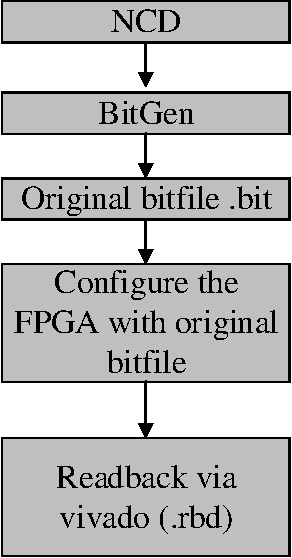
\includegraphics[scale = 0.5]{Figures/original-rbd.pdf}
   \caption{Procedure to extract the original .rbd file}
\label{fig:original-rbd}
\end{figure}

\begin{figure}[tb!]
 \centering
  \captionsetup{justification=centering}    
   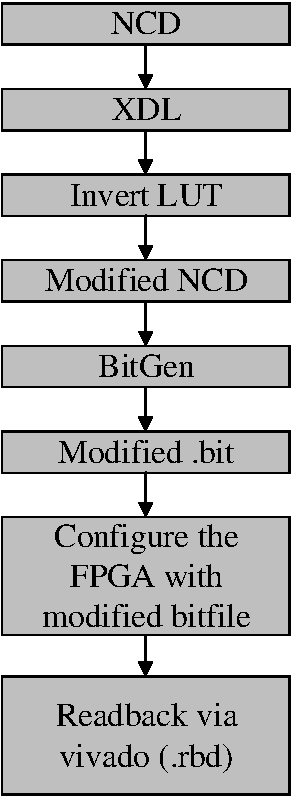
\includegraphics[scale = 0.5]{Figures/inverted-rbd.pdf}
   \caption{Procedure to extract the inverted LUT .rbd file}
\label{fig:inverted-rbd}
\end{figure}





\begin{algorithm}
\caption{Bits classification algorithm}
\begin{algorithmic}
\label{BCA}
\REQUIRE $.rbd$ $original$ $and$ $.rbd$ $inverted$ \\
%\textbf{Compute}\\ 
%\hspace{1.5cm}{$Original =  A $ $ \times $ $ B$ } \\
%\hspace{1.5cm}{$Faulty =  A $ $ \times $ $ B$ } \\
%\vspace{0.20 cm }
%\textbf{Stuck-at-1:}
\vspace{0.20 cm }

\IF{$Original$  $ = $ $ 0 $  $Inverted$ $==$ $0$}
\vspace{0.10 cm }

\STATE \textit{ NL0 = Not LUT bits at 0}
\vspace{0.10 cm }

\ELSIF{$Original$  $ = $ $ 0 $  $Inverted$ $==$ $1$}
\vspace{0.10 cm }

\STATE \textit{ L0 = LUT bits at 0}
\vspace{0.10 cm }

\ELSIF{$Original$  $ = $ $ 1 $  $Inverted$ $==$ $0$}
\vspace{0.10 cm }

\STATE \textit{ L1 =  LUT bits at 1}
\vspace{0.10 cm }

\ELSIF{$Original$  $ = $ $ 1 $  $Inverted$ $==$ $1$}
\vspace{0.10 cm }

\STATE \textit{ NL1 = Not LUT bits at 1}
\vspace{0.10 cm }




\ENDIF
\vspace{0.20 cm }

\end{algorithmic}
\end{algorithm}






\section{Experimental Results}
\label{Experimental Results}

In this section, we will discuss the result of emulation performed by flipping the bits at "1" and at "0." We experimented with the fifty different runs. Each run provides $6,144$ signatures further sub-divided into three separate groups.  The fault generation list is generated from the \textit{.rbd} file, extract the number of zeros and ones from the \textit{.rbd} file.

Table~\ref{AE}, and Table~\ref{ME} show the percentage of the zero signature, e.g., $00000000$ for adder and multiplier. The maximum number of zero signature observed for flip-at-0. The number of bits flipped observed; $65,750$ among them $150$ bits are critical bits with the statistical ratio of $0.22\%$ critical bits at $0$. The minimum number of zero signature observed for bits flip-at-1, with the total flipped bits are $1,356$ among $3,110,418$ non-BRAM bits. In this case, the critical bits at $1$ are $11.06\%$. 

Similarly, for the multiplier,  The number of bits flipped observed are $29,752$ with total non-BRAM(bits-at-0) are $56,771,430$ giving the statistical ratio of $0.50\%$ critical bits at $0$. The minimum number of zero signature observed for bits flip-at-1, with the total flipped bits are $1,664$ among $3,750,970$ non-BRAM bits. In this case, the critical bits at $1$ are $9.01\%$.


Then the emulation performed with the random fault injection, in which we randomly combined the bits-at-1, and the bits-at-0 and calculated the zero signature. As expected, the random injection zero-signature value should lower than the flip-at-0 and higher than the flip-at-1. The purpose of performing the random injection is to compare the result with the relative sensitivity results and experimentally prove that relative sensitivity of the bits produced results closer than the radiation experiment. The bit flip ratio observed in the random injection (flip-at-0 to flip-at-1) is $18.10$ for the adder as shown in Table~\ref{RI} and $15.15$ for the multiplier as shown in Table\ref{RIM}. This bit-flip information indicates that the bit flip in random mode is valid. Next, we performed the relative sensitivity experiment named SA-01, and SA-02.

In SA-01, we used the relative sensitivity concept that the  bits-at-1 are $2.11$ times more sensitive than the bit-at-0. In this emulation, we get the $1.87\%$ difference with the irradiation experiment for the adder and $1.58\%$ for the multiplier. The total bit flips we observed for adder are: $9,807$ among them $8,797$ flipped-at-0 and $1,010$ for flipped-at-1. Similarly, for the multiplier, the total bits flipped are $7,227$ among them $6,345$ flipped-at-0 and $882$ flipped-at-1. Both emulations give us the bit flipped ratio of $2.11$ proved that emulation setup is valid.

\begin{table}[tb!]
\center
\caption{Adder Emulation Tests Comparison.}

\label{AE}

\begin{tabular}{|c | c| c | c| c| c |} 
 \hline
Test & Zero Signature (\%) & Difference with Radiation (\%)   \\ 
\hline

 
 
 Flip@1& 49.048 &22.53   \\
 \hline
 Flip@0 & 62.801 & 2.095 \\ 
 \hline
 
 Random & 59.378 & 3.51  \\
 \hline
 SA-01 & 60.36 & 1.87 \\
 \hline
 SA-02 & 60.559 &1.47  \\
 \hline
 Radiation & 61.499 & 0  \\
 \hline
 
 
\end{tabular}
\end{table}


\begin{table}[tb!]
\center
\caption{Multiplier Emulation Tests Comparison.}

\label{ME}

\begin{tabular}{|c | c| c | c| c| c |} 
 \hline
Test & Zero Signature (\%) & Difference with Radiation (\%)   \\ 
\hline

 
 
 Flip@1& 62.069 &18.35   \\
 \hline
 Flip@0 & 76.066 & 1.93 \\ 
 \hline
 
 Random & 72.179 & 3.31  \\
 \hline
 SA-01 & 73.443 & 1.58 \\
 \hline
 SA-02 & 74.988 &  0.50\\
 \hline
 Radiation & 74.610 & 0  \\
 \hline
 
 
\end{tabular}
\end{table}



%We categorize the experiment in the five different categories based on the bits status, i.e., flipping the ( bits-at-1, bits-at-0, random, sensitivity based investigation that ones are more sensitive than zeros, and sensitivity based experiment consider bits feature). 
%Our emulation process is fundamentally different from the previous work published by our research group. The previous work was based on Viretx-V and fault injection was based on \textit{.ebc}, whereas this work is based on 
%the Artix-7 and fault emulation based on the \textit{.rbd} file details mentioned in section~\ref{SE-bits}. Inorder to do the fault emulation, we performed the experiment that reduce the time and the cost to perform the SEU emulation.




\begin{table}[tb!]
\center
\caption{Adder Random Injection Bits Information}

\label{RI}

\begin{tabular}{c c  c c   } 
 \hline
\multicolumn{2}{c}{Bit}     & Flip Ratio (Theoretical) &  Flip Ratio (Observed)   \\ 
%\hline
%& \multicolumn{1}{c}{ (Theoretical)} \\
%& & \multicolumn{1}{c}{observed} \\
 \hline
 
 Bits@0 & $57 411 982  $ & \multirow{2}{*}{18.45} & \multirow{2}{*}{18.10} \\
 %\hline
 Bits@1 & $3110418$  & &\\ 
 \hline
% 
% Bits@0 LUT & 2.06 &2.08 &2.096\\
% \hline
% Bits@1 LUT & 1.91 &1.92&1.91\\
 %\hline

% \hline
 
 
\end{tabular}
\end{table}


\begin{table}[tb!]
\center
\caption{Multiplier Random Injection Bits Information}

\label{RIM}

\begin{tabular}{c c  c c   } 
 \hline
\multicolumn{2}{c}{Bit}     & Flip Ratio (Theoretical) &  Flip Ratio (Observed)   \\ 
%\hline
%& \multicolumn{1}{c}{ (Theoretical)} \\
%& & \multicolumn{1}{c}{observed} \\
 \hline
 
 Bits@0 & $57 411 982  $ & \multirow{2}{*}{15.93} & \multirow{2}{*}{15.15} \\
 %\hline
 Bits@1 & $3110418$  & &\\ 
 \hline
% 
% Bits@0 LUT & 2.06 &2.08 &2.096\\
% \hline
% Bits@1 LUT & 1.91 &1.92&1.91\\
 %\hline

% \hline
 
 
\end{tabular}
\end{table}





Then, we further investigated the bits feature, i.e., bits belong to LUT and non-LUT bits. We used the bits relative sensitivity values shown in Table~\ref{RS}. The result we obtained by using this approach indicates only $1.47\%$ difference for adder and $0.50\%$ for multiplier suggest that by considering bits sensitivity with bits feature more realistic results can be achieved, and better fault emulation can be performed. 



%\begin{table}[tb!]
%\center
%\caption{Adder Emulation Tests Comparison.}
%
%\label{AE}
%
%\begin{tabular}{|c | c| c | c| c| c |} 
% \hline
%Test & Zero Signature (\%) & Difference with Radiation (\%)   \\ 
%\hline
%
% 
% 
% Flip@1& 49.048 &22.53   \\
% \hline
% Flip@0 & 62.801 & 2.095 \\ 
% \hline
% 
% Random & 59.378 & 3.51  \\
% \hline
% SA-01 & 60.36 & 1.87 \\
% \hline
% SA-02 & 60.559 &1.47  \\
% \hline
% Radiation & 61.499 & 0  \\
% \hline
% 
% 
%\end{tabular}
%\end{table}





We also measure the relative sensitivity (observed) and the bit flip information observed for this emulation setup shown in the Table~\ref{RS} to prove the bit flip emulation validity. Table~\ref{RSflipA} and~\ref{RSflipM} shows the bit flip information for the adder and multiplier respectively.


\begin{table}[tb!]
\center
\caption{Relative Sensitivity}

\label{RS}
\begin{tabular}{|c | c| c | c | } 
 \hline
Bits feature & \makecell*{Relative Sensitivity}  & \makecell*{Adder \\(Observed)} & \makecell*{Multiplier \\ (Observed)}  \\ 
%\hline
%& \multicolumn{1}{c}{ (Theoretical)} \\
%& & \multicolumn{1}{c}{observed} \\
 \hline
 
 Bits@0 non LUT & 1.00 & 1.00 & 1.00 \\
 \hline
 Bits@1 non LUT& 1.41  & 1.43&1.44\\ 
 \hline
 
 Bits@0 LUT & 2.06 &2.08 &2.09\\
 \hline
 Bits@1 LUT & 1.91 &1.92&1.91\\
 \hline

% \hline
 
 
\end{tabular}
\end{table}


















\begin{table}[tb!]
\center
\caption{Bit Flip Ratio Relative Sensitivity (Adder)}

\label{RSflipA}
\begin{tabular}{|c | c| c | c | } 
 \hline
Bits feature & \makecell*{Bit Flip)}  & \makecell*{Bit Flip Ratio\\(Total)} \\ 
%\hline
%& \multicolumn{1}{c}{ (Theoretical)} \\
%& & \multicolumn{1}{c}{observed} \\
 \hline
 
 Bits@0 non LUT & 5251  & 1.00  \\
 \hline
 Bits@1 non LUT& 236  & 1.43\\ 
 \hline
 
 Bits@0 LUT & 266 &2.08 \\
 \hline
 Bits@1 LUT & 245 &1.92\\
 \hline

% \hline
 
 
\end{tabular}
\end{table}



\begin{table}[tb!]
\center
\caption{Bit Flip Ratio Relative Sensitivity (Mull)}

\label{RSflipM}
\begin{tabular}{|c | c| c | c | } 
 \hline
Bits feature & \makecell*{Bit Flip}  & \makecell*{Bit Flip Ratio\\(Total)} \\ 
%\hline
%& \multicolumn{1}{c}{ (Theoretical)} \\
%& & \multicolumn{1}{c}{observed} \\
 \hline
 
 Bits@0 non LUT & 8833  & 1.00  \\
 \hline
 Bits@1 non LUT& 454  & 454\\ 
 \hline
 
 Bits@0 LUT & 603 &2.09\\
 \hline
 Bits@1 LUT & 553 &1.91\\
 \hline

% \hline
 
 
\end{tabular}
\end{table}







%
%\begin{equation}
%\label{eq:2}
%
%d
%\end{equation}

% \[
%    \text{Relative Sensitivity} =  \frac{x+y}{1 + \frac{y}{z+1}}
%\]

%\begin{equation} \label{eq:1}
%
%
%{Relative Sensitivity
%
%\end{equation}




%%\section{Fault Modeling}
%
%Once we get the signature from the emulation, validate all the bits flip information and zero signature validation.Next target is to drive a mathematical expression or model that can represent the high-level model that correspondence the low-level circuit faulty outputs. This model helps the designer to analyze the circuit and propose the necessary mitigation techniques at the earlier stage of the design. 
%
%
%
%\begin{algorithm}
%\caption{Generate a High-level Model of  Adder in Simulink}
%\begin{algorithmic}
%\REQUIRE $0\leq i \geq16$ \\
%\textbf{Compute}\\ 
%\hspace{1.5cm}{$Original =  A $ $ $+$ $ $ B$ } \\
%\hspace{1.5cm}{$Faulty =  A $ $ $+$ $ $ B$ } \\
%\vspace{0.20 cm }
%\textbf{Stuck-at-1:}
%\vspace{0.20 cm }
%
%\IF{$Original(i) == 1$ $and$  $Faulty (i) == 0 $}
%\vspace{0.10 cm }
%\STATE $Signature \leftarrow  \{$+$ 2^{i},$ $ $$zeros$$\{i-1\}\}$
%\vspace{0.10 cm }
%\ENDIF
%\vspace{0.20 cm }
%
%\textbf{Stuck-at-0:}
%\vspace{0.20 cm }
%\IF{$Original(i) == 0$ $and$  $Faulty (i) == 1 $}
%\vspace{0.10 cm }
%\STATE $Signature \leftarrow  \{$-$ 2^{i},$ $ $$zeros$$\{i-1\}\}$
%\vspace{0.10 cm }
%\ENDIF
%
%
%
%\vspace{0.20 cm }
%
%%\textbf{Stuck-at-0:}
%\vspace{0.20 cm }
%\IF {$Original$$-$$Faulty$  $==$ $MSB=1$ $and$ $1$}
%\vspace{0.10 cm }
%\STATE $Signature \leftarrow  \{$$Original-Faulty$$\}$
%\vspace{0.10 cm }
%\ENDIF
%
%
%
%
%%%\STATE $N \leftarrow -n$
%%%\ELSE
%%\STATE $X \leftarrow x$
%%\STATE $N \leftarrow n$
%%\ENDIF
%%\WHILE{$N \neq 0$}
%%\IF{$N$ is even}
%%\STATE $X \leftarrow X \times X$
%%\STATE $N \leftarrow N / 2$
%%\ELSE[$N$ is odd]
%%\STATE $y \leftarrow y \times X$
%%\STATE $N \leftarrow N - 1$
%%\ENDIF
%%\ENDWHILE
%\end{algorithmic}
%\end{algorithm}
%
%
%\begin{algorithm}
%\caption{Generate a High-level Model of  Multiplier in Simulink}
%\begin{algorithmic}
%\REQUIRE $ i = 16$  $bit$ $unsigned$ \\
%\textbf{Compute}\\ 
%\hspace{1.5cm}{$Original =  A $ $ \times $ $ B$ } \\
%\hspace{1.5cm}{$Faulty =  A $ $ \times $ $ B$ } \\
%\vspace{0.20 cm }
%\textbf{Stuck-at-1:}
%\vspace{0.20 cm }
%
%\IF{$Original$  $ - $  $Faulty$ $==$+$2^{i}$}
%\vspace{0.10 cm }
%\STATE $Signature \leftarrow  \{$+$ 2^{i}\}$
%\vspace{0.10 cm }
%%\ENDIF
%\vspace{0.20 cm }
%
%
%\ELSIF{$Original$  $ - $  $Faulty$ $==$ +$A$ $\times$ $2^{i}$ $or$ $ $+$B$ $\times$ $2^{i}$}
%\vspace{0.10 cm }
%\STATE $Signature \leftarrow  \{$+$  $A$ $ $ \times $ $2^{i} $ $ $or$ $ $ $+$ $B$ $ $ \times $ $2^{i}\}$
%
%
%\vspace{0.10 cm }
%\ENDIF
%\vspace{0.20 cm }
%
%\vspace{0.20 cm }
%\textbf{Stuck-at-0:}
%\vspace{0.20 cm }
%
%\IF{$Original$  $ - $  $Faulty$ $==$ -$2^{i}$}
%\vspace{0.10 cm }
%\STATE $Signature \leftarrow  \{$-$ 2^{i}\}$
%\vspace{0.10 cm }
%%\ENDIF
%\vspace{0.20 cm }
%
%
%\ELSIF{$Original$  $ - $  $Faulty$ $==$ -$A$ $\times$ $2^{i}$ $or$ $ $-$B$ $\times$ $2^{i}$}
%\vspace{0.10 cm }
%\STATE $Signature \leftarrow  \{$-$  $A$ $ $ \times $ $2^{i} $ $ $or$ $ $ $-$  $B$ $ $ \times $ $2^{i}\}$
%
%\vspace{0.10 cm }
%\ENDIF
%\vspace{0.20 cm }
%
%\end{algorithmic}
%\end{algorithm}
%
%\subsection{Adder Signature Fault Model}
%
%The adder is comprised of two 16-bits number. The adder signature is the 16-bit hexadecimal format with sign extension. The hexadecimal value comprises: first four from left are the signature hexadecimal representation, and the rest represent sign extension. The signature values with this simple expression shown in Table~\ref{adder signature format}.
%
%
%
%\begin{table}
%\center
%\caption{Adder Signature Format.}
%
%\label{adder signature format}
%
%\begin{tabular}{|c | c |} 
% \hline
%Decimal Format & Hexadecimal   \\ 
%\hline
%
% 
% 
% $16$& $00000010$    \\
% \hline
% $64$ & $00000040$  \\ 
% \hline
% 
% $128$ & $00000080$  \\
% \hline
% $-1024$ & $FFFFFC00$ \\
% \hline
% $-512$ & $FFFFFE00$ \\
% \hline
% $-8$ & $FFFFFFF8$   \\
% \hline
% 
% 
%\end{tabular}
%\end{table}
%
%
%
%
%\begin{equation}
%\label{eq:2}
%\pm±2\textsuperscript{i}    \hspace{0.5 cm} 0\leq i \geq15
%\end{equation}
%
%The Equation \ref{eq:2} can represent the adder high-level fault model. By using this equation, we can capture 99.99 \% of the signature. Table~\ref{adder signature format} shows two kinds of signature; positive signature and negative signature. The positive signature values can be modeled as \textbf{single stuck-at-one} model fault affecting an adder output bit $i$,  it adds $0$ when the target bit is at $1$ (flipped to $0$ in the faulty output). The signature computed can be expressed as $+2^{i}$. Consider the following example:
%
%
%%\rule{\linewidth}{1 pt} % A
%%\vskip-\baselineskip\vskip1.5pt % A+B
%%\rule{\linewidth}{0.1pt} %B
%\vspace{ 0.1 cm}
%\hspace{-0.3 cm}\textbf{Example:}
%\hrule height 2pt width \hsize \kern 1pt \hrule width \hsize height 1pt
%
%\vspace{0.2 cm}
%$Original$ $=$ $24$; $binary $ $ equivalent$ $11000$ \\
%
%\hspace{-0.15cm} $Faulty$ $=$ $8$; $binary $ $ equivalent$ $01000$ \\
%
%$fourth$ $bit$ $flipped$ $from$ $"1"$ $to$ $"0"$
%
%$By$ $using$ $equation$ \ref{eq:1}: \\
%
%$signature$ $=$ $8$ - $24$ $==$ $8$ $+$ $(-24)$ $=$ $16$ \\
%
%$4^{th}$ $ bit $ $flipped$; $i$  $=$ $4$, $2^{4}$ $=$ $16$
%\vspace{0.01cm}
%\hrule height 2pt width \hsize \kern 1pt \hrule width \hsize height 1pt
%
%\vspace{0.25 cm}
%
%Similarly, for the negative signature values can be modeled as single stuck-at zero model - fault affecting an adder output bit $i$, it adds $0$ when the target bit is at $0$ (flipped to $1$ in the faulty output), it adds $-2i$ to the adder output. We also observed that few signatures that didn't follow the rule number one could be modeled with: 
%
%Rule 2: if the signature cannot be modeled with the Equation~\ref{eq:1}, if the arithmetic signature values expressed in binary format and contained exactly two bits@1, including one at the MSB.
%
%\hspace{-0.3 cm}\textbf{Example valid signatures for rule \# 02:}
%\hrule height 2pt width \hsize \kern 1pt \hrule width \hsize height 1pt
%\begin{center}
%$1010 0000 0000 0000$ \\
%$1000 1000 0000 0000$ \\
%$1000 1000 0000 0000$ \\
%$1000 0000 0000 0100$ \\
%$1000 0000 0000 0001$ \\
%\end{center}
%\hrule height 2pt width \hsize \kern 1pt \hrule width \hsize height 1pt
%
%
%
%
%
%
%
%
%\subsection{Multiplier Signature Fault Model}
%
%For the 8 - bit multiplier two modeling rules have been formulated:
%
%\textbf{Rule \# 01:} This rule defines the signature can be expressed by the Equation \ref{eq:1} that represent the stuck-at-1 and stuck-at-0 fault model, when the multiplier behaves as the bit flipped occur at the output of the multiplier. 
%
%\textbf{Rule \# 02:}The rule number two defines the format of the signature obtained when a bit flipped cause the multiplier to behave as if when an input bit is either stuck-at-0 or stuck-at-1 can be represented \{$-$$A$ $\times$ $2^{i}$ $or$  $-$$B$ $\times$ $2^{i}$ \}, \{$+$$A$ $\times$ $2^{i}$ $or$  $+$$B$ $\times$ $2^{i}$ \} respectively.
\section{Conclusions}


In this work, sensitivity of the configuration bits has been considered along with the bits feature to
produce results as close as possible to those obtained by the accelerated tests. 



\label{Conclusion}

